\documentclass[border=2pt]{standalone}
\usepackage[T1]{fontenc}
\usepackage{helvet}
\renewcommand{\familydefault}{\sfdefault}
\usepackage{tikz}
\usetikzlibrary{arrows.meta,calc}

\definecolor{ink}{HTML}{0F172A}
\definecolor{muted}{HTML}{64748B}
\definecolor{line}{HTML}{CBD5E1}
\definecolor{green}{HTML}{16A34A}
\definecolor{amber}{HTML}{CA8A04}
\definecolor{gray}{HTML}{94A3B8}

\newcommand{\panelhead}[1]{{\fontsize{6.2}{7.4}\selectfont\bfseries\color{muted}#1}}
\newcommand{\body}[1]{{\fontsize{6.0}{7.3}\selectfont\color{ink}#1}}
\newcommand{\tile}[4]{%
  \node[fill=#1, rounded corners=0.7mm, minimum width=0.74cm, minimum height=0.74cm,
        inner sep=0pt, text=white, font=\bfseries\fontsize{7.6}{9}\selectfont]
       at (#2,#3) {#4};}

\begin{document}
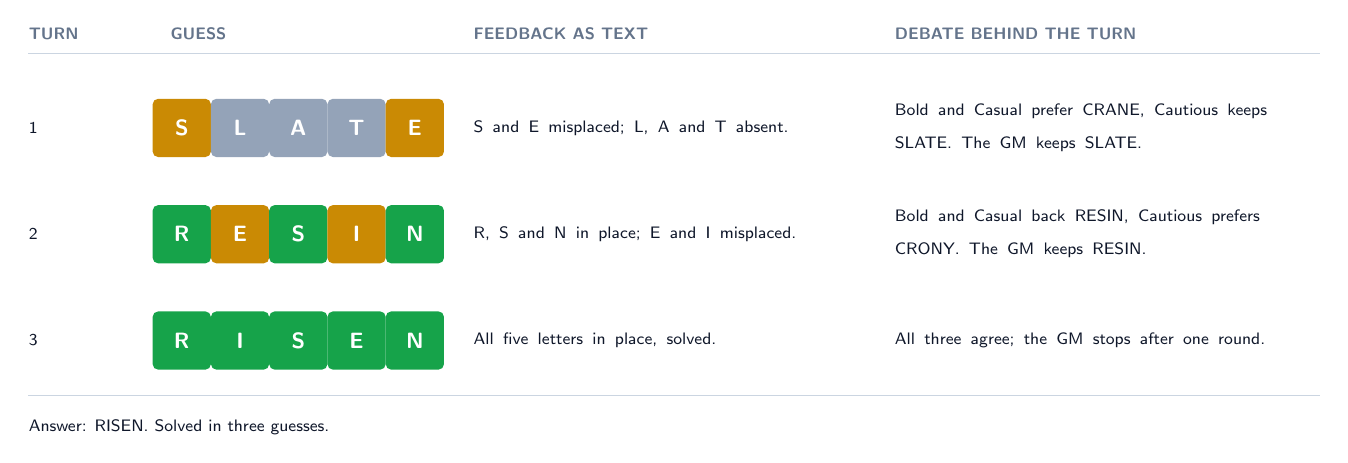
\begin{tikzpicture}[x=1cm,y=1cm]

% headers
\node[anchor=west, inner sep=0] at (0.30,5.55) {\panelhead{TURN}};
\node[anchor=west, inner sep=0] at (2.10,5.55) {\panelhead{GUESS}};
\node[anchor=west, inner sep=0] at (5.95,5.55) {\panelhead{FEEDBACK AS TEXT}};
\node[anchor=west, inner sep=0] at (11.30,5.55) {\panelhead{DEBATE BEHIND THE TURN}};
\draw[line, line width=0.4pt] (0.30,5.30) -- (16.70,5.30);

% turn 1
\node[anchor=west, inner sep=0] at (0.30,4.35) {\body{1}};
\tile{amber}{2.25}{4.35}{S}
\tile{gray}{2.99}{4.35}{L}
\tile{gray}{3.73}{4.35}{A}
\tile{gray}{4.47}{4.35}{T}
\tile{amber}{5.21}{4.35}{E}
\node[anchor=west, inner sep=0, text width=5.0cm, align=left] at (5.95,4.35) {\body{S and E misplaced; L, A and T absent.}};
\node[anchor=west, inner sep=0, text width=5.3cm, align=left] at (11.30,4.35) {\body{Bold and Casual prefer CRANE, Cautious keeps SLATE. The GM keeps SLATE.}};

% turn 2
\node[anchor=west, inner sep=0] at (0.30,3.00) {\body{2}};
\tile{green}{2.25}{3.00}{R}
\tile{amber}{2.99}{3.00}{E}
\tile{green}{3.73}{3.00}{S}
\tile{amber}{4.47}{3.00}{I}
\tile{green}{5.21}{3.00}{N}
\node[anchor=west, inner sep=0, text width=5.0cm, align=left] at (5.95,3.00) {\body{R, S and N in place; E and I misplaced.}};
\node[anchor=west, inner sep=0, text width=5.3cm, align=left] at (11.30,3.00) {\body{Bold and Casual back RESIN, Cautious prefers CRONY. The GM keeps RESIN.}};

% turn 3
\node[anchor=west, inner sep=0] at (0.30,1.65) {\body{3}};
\tile{green}{2.25}{1.65}{R}
\tile{green}{2.99}{1.65}{I}
\tile{green}{3.73}{1.65}{S}
\tile{green}{4.47}{1.65}{E}
\tile{green}{5.21}{1.65}{N}
\node[anchor=west, inner sep=0, text width=5.0cm, align=left] at (5.95,1.65) {\body{All five letters in place, solved.}};
\node[anchor=west, inner sep=0, text width=5.3cm, align=left] at (11.30,1.65) {\body{All three agree; the GM stops after one round.}};

% footer rule
\draw[line, line width=0.4pt] (0.30,0.95) -- (16.70,0.95);
\node[anchor=west, inner sep=0] at (0.30,0.55) {\body{Answer: RISEN. Solved in three guesses.}};

\end{tikzpicture}
\end{document}
